When analyzing the resulting circuit of longer ($\ge$ 5 steps) SQWs a pattern starts to emerge in the resulting circuit. This pattern also is repeated in the same amount as the number of steps in the quantum walk. This leads us to believe that this operator is capable of representing both the increment and decrement layers of the evolution operator, or at least approximate the SQW evolution operator.

The following is a ZX-diagram representation of the above-mentioned operator.

\begin{align}
    \tikzfig{sqw-pattern-standard}
\end{align}

Where:

\begin{equation}
    \alpha_n = \pm \frac{\pi}{4}
\end{equation}
\begin{equation}   
    \beta_n = \frac{2\pi}{3} + n\pi 
\end{equation}

with $n=0$ or $n=1$.


There is also a slight variation of this operator, where a CNOT gate between the first and last qubit appears right after the $\beta_1$ Z-spider.


\begin{align}
    \tikzfig{sqw-pattern-variation}
\end{align}

This operator by itself doesn't fully capture the SQW we started with, but in conjunction with a set of gates in the beginning and the end of the circuit it represents the exact same tensor as the original circuit. 


% Possivelmente utilizar o seguinte para as desvantagens

These initial and final set of gates do not seem to follow any sort of structure or reason for the gates that are used. However, the initial segment of the circuit always appears to have 4 rotations combined with a seemingly random arrangement of other phase-less gates.


This operator appeared when optimizing the 3 qubit Staggered Quantum Walk, however if one follows the way this operator is constructed this can be generalized for an $n$ qubit implementation of this operator.

Thus yielding the following operator, in the form of a ZX-diagram:

\begin{align}
    \tikzfig{sqw-pattern-generalization}
\end{align}

This operator is constructed by entangling the first and last qubit and placing them in superposition. This is achieved by the XCX-gate (which is a CNOT with a hadamard on both sides of the control), then it is followed by a CNOT gate between the first and last qubit and a rotation over the X-axis on the first qubit. Afterwards a ladder of XCX-gates starting with the first qubit and the $n-1^{th}$ qubit and descending all the way to the second. This is then followed by a rotation over the Z-axis along with a X-axis rotation. Then a CNOT is applied to the first and last qubit, following this there's a X-axis rotation and a XCX-gate over the first qubit and the $n-1^{th}$ qubit. Then there's the second Z-axis rotation subsequently followed by the same ladder of XCX-gates, although this time it starts between the first and the $n-2^{th}$ qubit and descending all the way to the second. Finishing off with the last X-axis rotation.

The logic behind this operator is creating a uniform distribution over a certain number of states, applying a rotation to that uniform distribution that makes some states more likely than others and then spreading these probabilities over the other states using CNOT gates.

When we take the nature of this operator into consideration it is obvious why it only shows up in SQWs over a certain length. The classical operator for the SQW using the increment and decrement layers needs to be repeated a number of times to be able to spread the probabilities' distribution over the whole state space. This is something that this alternative operator does on the first layer, thus it cannot approximate SQWs with a few steps as well as it can for longer quantum walks.

\subsection{Advantages of this alternative operator}

Besides this, this new operator has a whole set of advantages. The first one being the total amount of gates needed to represent the evolution of the quantum walk. With the number of qubits in the SQW increasing so does the cost of the increment and decrement layers, as an $n$ qubit SQW needs to implement MCX gates with $n-1$ controls. These MCX gates need to then be expanded into it's basic gates representation \cite{gate-decomp}. All the while this new operator at most utilizes gates controlled with at most 1 qubit. Also, when we go from an $n$ qubit to a $n+1$ qubit quantum walk all that needs to be done is add two more XCX-gates, one to each ladder of XCX-gates, the same can't be said about the evolution operator based on increment and decrement operators. 

This leads to this alternative operator being much more efficient when it comes to the total amount of gates used, leading to lower depth circuits and in turn less error-prone.



Just by itself this operator is capable of approximating the evolution of a SQW. Although the approximation isn't perfect it can yield results with a distribution of probabilities quite similar to the original implementation of the SQW.
\begin{align}
    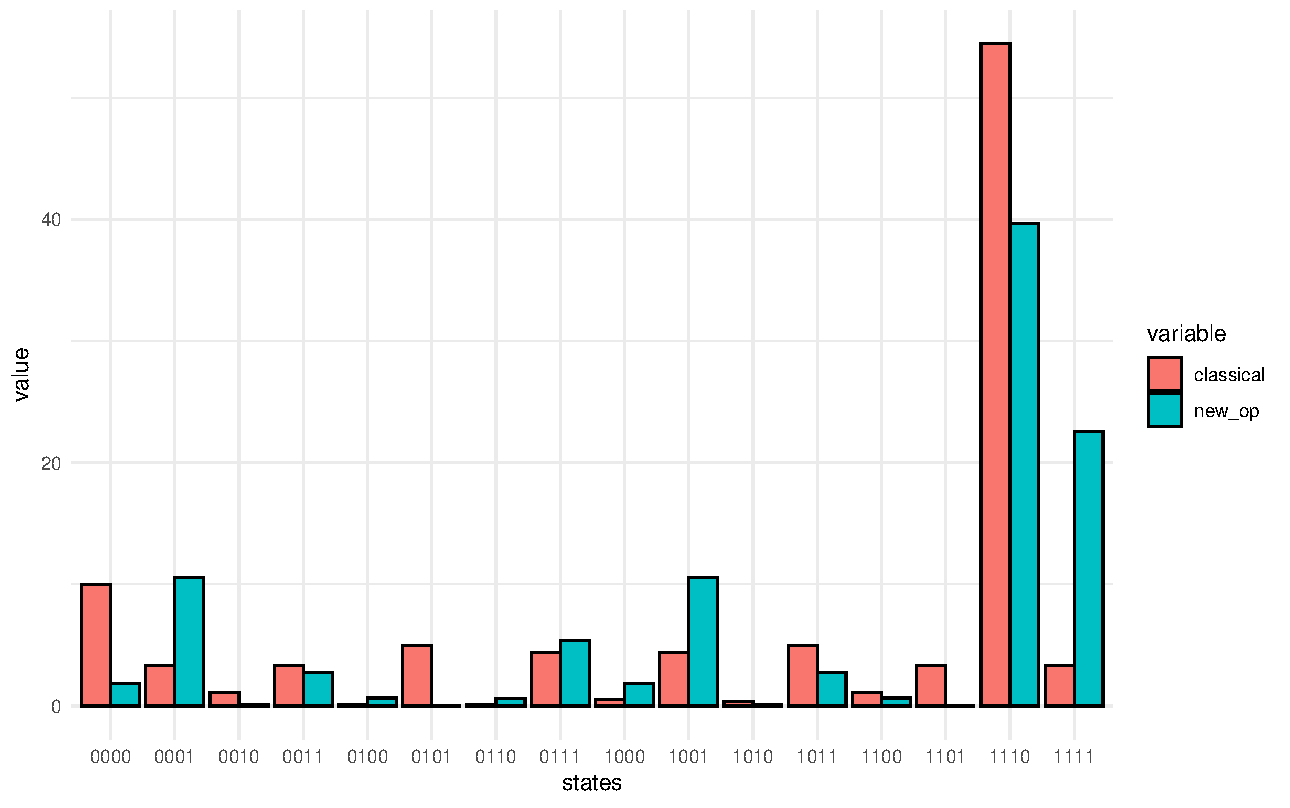
\includegraphics[width=0.7\linewidth]{figures/4step.pdf}
\end{align}

One particular advantage of this specific implementation of the evolution operator is that it can work quite well on QPUs that have a very limited connectivity. This is due to the fact that all the qubits used in the SQW only need to have a strong connectivity with only the first qubit, thus minimizing possible errors occurring from having to operate on two qubits with poor connectivity.

\subsection{Disadvantages of this alternative operator}

Although this operator presents itself with a plethora of advantages it also presents a lot of challenges when it comes to actually using it. This is due mostly to the lack of reason as to which values should the $\alpha_n$ and $\beta_n$ parameters be. Or even, if these parameters should change with the change of how many qubits are used in the Staggered Quantum Walk. When optimizing the 3 qubit implementation of the SQW the resulting parameters did not seem to follow any reasonable pattern. 

There doesn't seem to be a way to determine which values these parameters should take to approximate a given SQW.

Also, there doesn't seem to be a guarantee as to if the next step of the SQW will be able to be approximated with the already established parameters, this can lead to sub-par approximations of the Staggered Quantum Walk.











